\section{Reachability Analysis on Hybrid Systems}

\subsection{Hybrid Automata}

Hybrid systems are a class of dynamical systems exhibiting both continuous flow and discrete jumps. They are usually systems composed of a discrete controller interacting with a physical environment. A popular class of formal models for hybrid systems are called \emph{hybrid automata}~\cite{}, whose definition is given as follows.

\begin{defn}
 A \emph{hybrid automaton} is defined by a tuple $\mathcal{A} = \tupleof{\loc, \var, \flow, \trans, \inv, \init}$ such that
 \begin{itemize}[-]
  \item $\loc$ is a finite set which consists of all discrete locations (or modes) of the system,
  
  \item $\var$ is a finite set which contains all continuous variables of the system,
  
  \item $\flow$ is a function associating each location a continuous dynamics which is defined by an ODE,
  
  \item $\trans$ consists of finitely many discrete jumps among the locations. A jump from $\ell$ to $\ell'$ is defined by a tuple $\tupleof{\ell, G, R, \ell'}$ such that $G\subseteq \reals^{|\var|}$, $R: \reals^{|\var|}\rightarrow \reals^{|\var|}$ are called the \emph{guard} and \emph{reset} respectively. The jump is enabled, i.e., allowed to take place, only if the guard $G$ is satisfied by the variable values. After the jump is made, the variable values are reassigned according to the reset $R$.
  
  \item $\inv$ is a function that defines a valid variable value range $\inv(\ell) \subseteq \reals^{|\var|}$ for each location $\ell \in \loc$,
  
  \item $\init$ is a set which contains all initial states of the system.
 \end{itemize}
\end{defn}

\begin{example}
 Figure~\ref{fig:thermostat} shows the hybrid automaton for a thermostat. It has two modes for the ``on'' and ``off'' states of the heater. The room temperature is denoted by the variable $x$. The system regulates the temperature between $15$ and $25$ by switching on or off the heater. When the heater is on, the temperature rises according to the ODE $\dot{x} = K(h-x)$. When it is off, the temperature drops according to $\dot{x} = -Kx$. The thermostat nondeterministically switches off the heater when the temperature is between $23$ and $25$, and on the other hand nondeterministically switches on the heater when the temperature is between $15$ and $17$.
\end{example}

\begin{minipage}{0.48\textwidth}
 \centering
 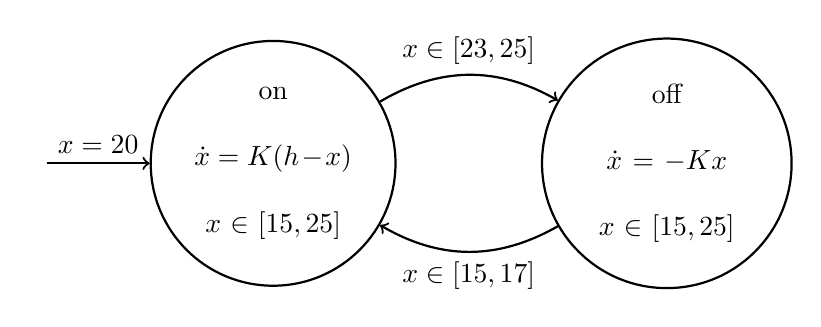
\begin{tikzpicture}
  \node[draw, circle, text width=2cm, thick, text centered] (l1) at (-2.5,0) {on \\ \ \\ $\dot{x} = K(h-x)$ \\ \ \\ $x \in [15, 25]$};
  \node[draw, circle, text width=2cm, thick, text centered] (l2) at (2.5,0) {off \\ \ \\ $\dot{x} = -Kx$ \\ \ \\ $x \in [15, 25]$};
  \node (init) at (-5.5,0) {};
  \path[->, thick] (l1) edge[bend left] node[above] {$x\in [23,25]$} (l2);
  \path[->, thick] (l2) edge[bend left] node[below] {$x\in [15,17]$} (l1);
  \path[->, thick] (init) edge node[above] {$x = 20$} (l1);
 \end{tikzpicture}
 \captionof{figure}{Hybrid automaton of a thermostat}\label{fig:thermostat}
\end{minipage}
\hspace{1ex}
\begin{minipage}{0.48\textwidth}
\end{minipage}

\subsection{Reachability Analysis}







